\section{Models}

This section describes the models in more detail.

\subsection{Target Architecture}
The following image depicts our target architecture developed for our experiments.

\begin{figure}[ht]
\centering
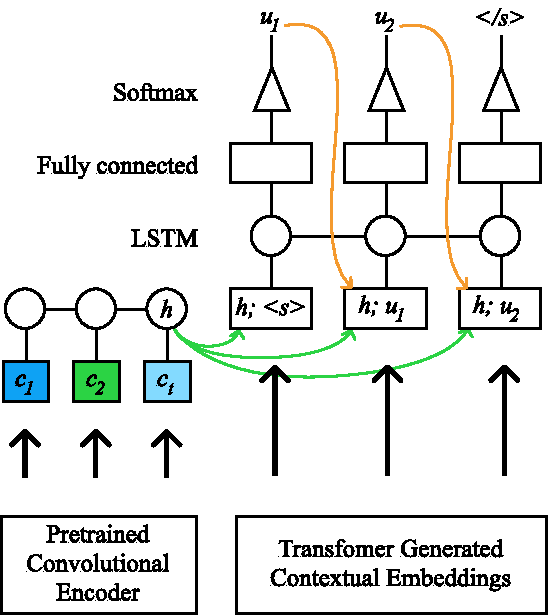
\includegraphics[width=\columnwidth]{assets/target_architecture.pdf}
\caption[Target Architecture]
{Target architecture with pretrained convolutional encoder and transformer generated contextual word embeddings.}
\label{overview}
\end{figure}

\par
The above architecture consists of three core components. The pretrained convolutional encoder is our method for extracting rich color embeddings. This could be any pretrained convolutional model such as \texttt{VGG19} or \texttt{Resnet152}, it just requires that we use one of the last hidden layers before the softmax projection as our encode color embeddings. We use the last layer of \texttt{ResNet18} in our experiments.

\par
The transformer generated contextual embeddings are any word embeddings generated by a transformer. This could be embeddings generated by \texttt{ELECTRA}, \texttt{XLNet}, \texttt{BERT} or any other transformer variants. These are used to encode the words into a semantic vector space where their project will be dependent on their context. Some descriptions are single words, thus contextual information will not be encoded.

\par
The generated color and contextual word embeddings are then brought together using a standard sequence-to-sequence architecture. The color embeddings are sent through an RNN unit such as a Gated Recurrent Unit or Long Short Term Memory Unit. The target color is sent through the RNN layer last so that it’s information encoded in the hidden state is \emph{closest} to the decoder. The decoder, another RNN unit,  then takes the hidden encoder's last hidden layer input and starts to decode the input utterance. For each timestep of the decoder we concatenate the target colors embedding, generated by the \texttt{ResNet18}, with the input word. Once the output RNN reaches its specified stop token we stop generating text.

\subsection{Experiment Setup}
To address our hypotheses we use different model compositions which are based on our target architecture.

\textbf{Baseline}:
As a baseline model, we use our implementation of the encoder-decoder architecture model based on a single layer of GRU for both the encoder and decoder. The colors are encoded using Fourier transformation.

\textbf{Part one}:
We use Fourier encoded context colors with pretrained and contextual embeddings from the following transformer models: \texttt{BERT}, \texttt{XLNet}, \texttt{ELECTRA}, \texttt{RoBERTa}.

\textbf{Part two}:
We use \texttt{ResNet} for contextual color representation while keeping the same model embeddings.

\textbf{Part three}:
We build on part two and combine different hidden layers of the transformer models. Namely, we concatenate the last four hidden layers, sum the last four hidden layers and extract the second-to-last hidden layer.